\documentclass[answers]{exam}
\usepackage{graphicx}
\usepackage{wrapfig}
\usepackage[utf8]{inputenc}

\title{PSYCH 260-BBH 203 Exam 1}
\author{}
\date{September 25, 2015}

\pagestyle{headandfoot}
\firstpageheader{PSY 260-BBH 203}{Section 002}{Exam 1}
\runningheader{PSY 260-BBH 203}{Section 002}{Exam 1}
\firstpagefooter{}{Page \thepage\ of \numpages}{}
\runningfooter{}{Page \thepage\ of \numpages}{}

\begin{document}
\maketitle

\begin{center}
  \fbox{\fbox{\parbox{5.5in}{\centering
        Answer the questions using the Scantron form.}}}
\end{center}
\vspace{0.1in}
\makebox[\textwidth]{Name:\enspace\hrulefill}

\newpage

\section{Main}

\begin{figure}[h]
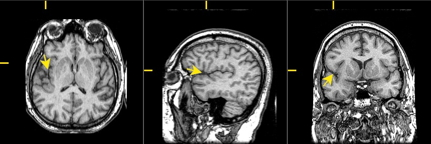
\includegraphics[width=0.80\textwidth]{img/three-brains.jpg}
\centering
\end{figure}

\begin{questions}

\question What plane of section is represented in the left panel?
\begin{choices}
\choice Coronal
\choice Sagittal
\correctchoice Axial/horizontal
\choice Dorsal
\end{choices}

\question What plane of section is represented in the middle panel?
\begin{choices}
\choice Coronal
\correctchoice Sagittal
\choice Axial/horizontal
\choice Dorsal
\end{choices}

\question What plane of section is represented in the right panel?
\begin{choices}
\correctchoice Coronal
\choice Sagittal
\choice Axial/horizontal
\choice Dorsal
\end{choices}

\question What fissure or sulcus is represented in the figures?
\begin{choices}
\correctchoice Lateral fissure
\choice Superior temporal sulcus
\choice Central sulcus
\choice Longitudinal fissure
\end{choices}

\newpage

\begin{center}
Identify the structures labeled in the figure below.
\end{center}

\begin{figure}[h]
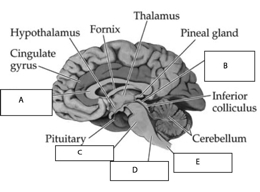
\includegraphics[width=0.50\textwidth]{img/label-sagittal.jpg}
\centering
\end{figure}

\question Spinal cord
\question Superior colliculus
\question Corpus callosum
\question Pons
\question Medulla oblongata 

\begin{center}
Identify anatomical links between structures in the following questions.
\end{center}

\question Motor cortex
\begin{choices}
\choice Temporal lobe
\correctchoice Frontal lobe
\choice Hypothalamus
\choice Basal ganglia
\choice Parietal lobe
\end{choices}

\question Auditory cortex
\begin{choices}
\correctchoice Temporal lobe
\choice Frontal lobe
\choice Hypothalamus
\choice Basal ganglia
\choice Parietal lobe
\end{choices}

\question Pituitary gland
\begin{choices}
\choice Temporal lobe
\choice Frontal lobe
\correctchoice Hypothalamus
\choice Basal ganglia
\choice Parietal lobe
\end{choices}

\question Somatosensory cortex
\begin{choices}
\choice Temporal lobe
\choice Frontal lobe
\choice Hypothalamus
\choice Basal ganglia
\correctchoice Parietal lobe
\end{choices}

\question Caudate nucleus
\begin{choices}
\choice Temporal lobe
\choice Frontal lobe
\choice Hypothalamus
\correctchoice Basal ganglia
\choice Parietal lobe
\end{choices}

\begin{center}
Match the structure with one of its primary functions in the following questions.
\end{center}

\question Hypothalamus
\begin{choices}
\correctchoice Sexual behavior
\choice Metabolic, physical support of neurons
\choice Sensory relay
\choice Memory storage and retrieval
\choice CNS protection
\end{choices}

\question Dura mater
\begin{choices}
\choice Metabolic, physical support of neurons
\choice Sensory relay
\choice Preparation for action
\choice Memory storage and retrieval
\correctchoice CNS protection
\end{choices}

\question Thalamus
\begin{choices}
\choice Sexual behavior
\choice Metabolic, physical support of neurons
\correctchoice Sensory relay
\choice Preparation for action
\choice Memory storage and retrieval
\end{choices}

\newpage

\question{Hippocampus}
\begin{choices}
\choice Sexual behavior
\choice Metabolic, physical support of neurons
\choice Sensory relay
\choice Preparation for action
\correctchoice Memory storage and retrieval
\end{choices}

\question{Sympathetic nervous system}
\begin{choices}
\choice Sexual behavior
\choice Metabolic, physical support of neurons
\choice Sensory relay
\correctchoice Preparation for action
\choice Memory storage and retrieval
\end{choices}

\question Which early Roman figure observed that head injuries caused mental and behavioral impairments?
\begin{choices}
\correctchoice Galen
\choice Aristotle 
\choice Vesalius 
\choice Da Vinci
\end{choices}

\question Natural philosophers in the middle ages thought that fluid from these structures inflated the muscles.
\begin{choices}
\choice Astrocytes
\choice Meninges
\correctchoice Cerebral ventricles
\choice Circle of Willis
\end{choices}

\question If you were interested in answering a question about how the human frontal and parietal lobes, as broad regions, respond to stimuli that change every 250 milliseconds, which of the following techniques would you use?
\begin{choices}
\correctchoice ERP
\choice Multi-unit recording 
\choice MRI
\choice Naturally occurring lesions
\end{choices}


\question \fillin, a type of glial cell, help regulate local blood oxygen levels in response to neuronal activity. These cells thus contribute to the signal measured by \fillin.
\begin{choices}
\choice oligodendrocytes; MEG
\choice Schwann cells; structural MRI
\correctchoice astrocytes; functional MRI
\choice microglia; structural and functional MRI
\end{choices}

\newpage

\question The layers of the meninges are organized in which of the following order, from dorsal (closest to bone) to ventral (closest to cortex)?
\begin{choices}
\choice Arachnoid membrane; Pia mater; Subarachnoid space; Dura mater
\correctchoice Dura mater; Arachnoid membrane; Subarachnoid space, Pia mater
\choice Pia mater; Subarachnoid space; Arachnoid membrane, Dura mater
\choice Subarachnoid space; Pia mater; Dura mater; Arachnoid membrane 
\end{choices}

\question Which of the following statements regarding the blood/brain barrier is NOT true?
\begin{choices}
\choice Active transport of molecules across the membrane is typically required 
\choice Blood vessel endothelial cells are tightly packed
\choice The entirety of the nervous system is protected by the barrier 
\correctchoice Microglia are the primary cell type that comprises the barrier
\end{choices}

\question The mesencephalon is another term for the \fillin; it contains the tectum and tegmentum. 
\begin{choices}
\correctchoice Midbrain 
\choice Forebrain
\choice Hindbrain
\choice Cerebellum 
\end{choices}

\question Which structure, located caudal to the fourth ventricle and contiguous with the spinal cord, controls many basic involuntary functions such as cardiovascular regulation?
\begin{choices}
\choice Superior colliculus 
\correctchoice Medulla oblongata 
\choice Pineal gland
\choice Fornix 
\end{choices}

\question The neurotransmitters dopamine, norepinephrine, and serotonin originate from nuclei clustered in which midbrain region? 
\begin{choices}
\choice Basal ganglia
\choice Lateral geniculate nucleus 
\correctchoice Tegmentum 
\choice Medial frontal cortex
\end{choices}

\question The hypothalamus is NOT responsible for which of the following functions?
\begin{choices}
\choice Fleeing 
\choice Feeding 
\choice Fighting 
\correctchoice Falling
\end{choices}

\question Which of the following marks the anterior boundary of the parietal lobe? 
\begin{choices}
\choice Lateral fissure 
\choice Longitudinal fissure 
\correctchoice Central sulcus 
\choice Inferior temporal gyrus 
\end{choices} 

\newpage

\question This type of myelinating cell, found in the \fillin, ensheaths many neurons at once.
\begin{choices}
\choice Astrocytes; PNS 
\correctchoice Oligodendrocytes; CNS 
\choice Schwann cells; CNS 
\choice Schwann cells; PNS  
\end{choices}

\question Nodes of Ranvier, or gaps in the myelination of an axon, serve which purpose? 
\begin{choices}
\correctchoice Increase the speed of propagation
\choice Allow space in the axon for neurotransmitter release
\choice Provide structural support to the neuron 
\choice Combine input from different dendrites 
\end{choices}

\question When a neuron is “at rest,” which of the following ions are more heavily concentrated \emph{outside} of the cell?
\begin{choices}
\correctchoice Na+ and Cl-
\choice K+ and A-
\choice Na+ and K+
\choice Cl- and A-  
\end{choices}

\question Which of the following is a characteristic of a neuron’s \emph{relative} refractory period?
\begin{choices}
\choice Na+ channels are either open or inactive
\correctchoice Very strong stimulation is required to generate an action potential 
\choice All types of ions are able to flow freely across the post-synaptic membrane 
\choice Action potentials generated during this time vary in size 
\end{choices}

\question What does the practice of trephining suggest? 
\begin{choices}
\choice Those who practiced the technique knew that the inner regions of the brain were filled with fluid
\choice Head injury impairs both behavior and thinking 
\choice Electrical stimulation changes behavior
\correctchoice Ancient practitioners thought that there was a link between the brain and mental function
\end{choices}

\question When a neuron's membrane potential reaches threshold \fillin.
\begin{choices}
\choice voltage-gated K+ channels close 
\choice voltage-gated Na+ channels close and inactivate
\choice the Na/K pump works even harder to keep the concentration balance.
\correctchoice voltage-gated Na+ channels open
\end{choices}

\newpage

\question This part of the cell functions as the neuron’s “antennae” by serving as the primary place for receiving input.
\begin{choices}
\choice Axon
\choice Soma
\correctchoice Dendrites
\choice Terminal Buttons
\end{choices}

\question During the rising phase of the action potential, \fillin channels \fillin.
\begin{choices}
\choice Ligand-gated K+ channels; close
\choice Voltage-gated Na+ channels; close
\correctchoice Voltage-gated Na+ channels; open
\choice Voltage-gated K+ channels; close
\end{choices}

\question During the \emph{falling} phase of the action potential, \fillin ions \fillin.
\begin{choices}
\correctchoice K+; flow out
\choice Na+; flow out
\choice K+; flow in
\choice Na+; flow in
\end{choices}

\question Neurons ensheathed in myelin conduct action potentials \fillin than those without myelin.
\begin{choices}
\choice more slowly
\correctchoice more quickly
\choice more slowly and efficiently
\choice more quickly, but less efficiently
\end{choices}

\section{Bonus}

\question What is NOT true about astrocytes?
\begin{choices}
\correctchoice They are present in the brain but not in the spinal cord
\choice They are the most numerous type of neuroglia cells
\choice They provide metabolic support for neurons
\choice They contribute to the blood/brain barrier
\end{choices}

\question Chloride ions would flow \fillin along their concentration gradient. This moves the neuron \fillin its firing threshold.
\begin{choices}
\correctchoice Inward; farther from
\choice Inward; closer to
\choice Outward; farther from
\choice Outward; closer to
\end{choices}

\newpage

\question A toxin found in Japanese pufferfish blocks voltage-gated Na+ channels. Applying such a toxin to neurons would have what effect?
\begin{choices}
\choice Slower falling phase of the action potential.
\choice Increasing the concentration of Na+ inside the cell.
\choice K+ ions would accelerate their flow to compensate.
\correctchoice Action potentials would be abolished.
\end{choices}

\question The striatum is a term for the \fillin and the \fillin.
\begin{choices}
\choice{hypothalamus; thalamus}
\correctchoice{caudate nucleus; putamen}
\choice{hippocampus; amygdala}
\choice{superior colliculus; inferior colliculus}
\end{choices} 

\end{questions}
\end{document}